\section{Exploratory Data Analysis}
\label{sec:explorator_data_analysis}
Data are collected from official statistical sources, primarily the Italian National Institute of Statistics (ISTAT), including the ISTAT Data Warehouse, the Permanent Census of Population and Housing, and \textit{Demografia in cifre}. Additional information was obtained from Eurostat and \textit{Il Sole 24 Ore, Qualità della vita} dataset.\\

This study focuses on 107 Italian provinces. For each of them, the data includes a total of 47 variables, representing different socio-economic measurements\footnote{The complete list of variables and their description is presented in Appendix A.}. \\
Since we want to analyze how ECEC services influence the women's labor market, our response variable is the women's employment rate.
Figure~\ref{fig:heatmap1} shows the spatial distribution of \texttt{fem\_empl\_rate}, defined as the ratio between the number of working women of working age (15-64 years old) and the total number of women of working age, and \texttt{coverage}, defined as the number of available children services over the number of children (0-2 years old):

\begin{figure}[h]
    \centering
    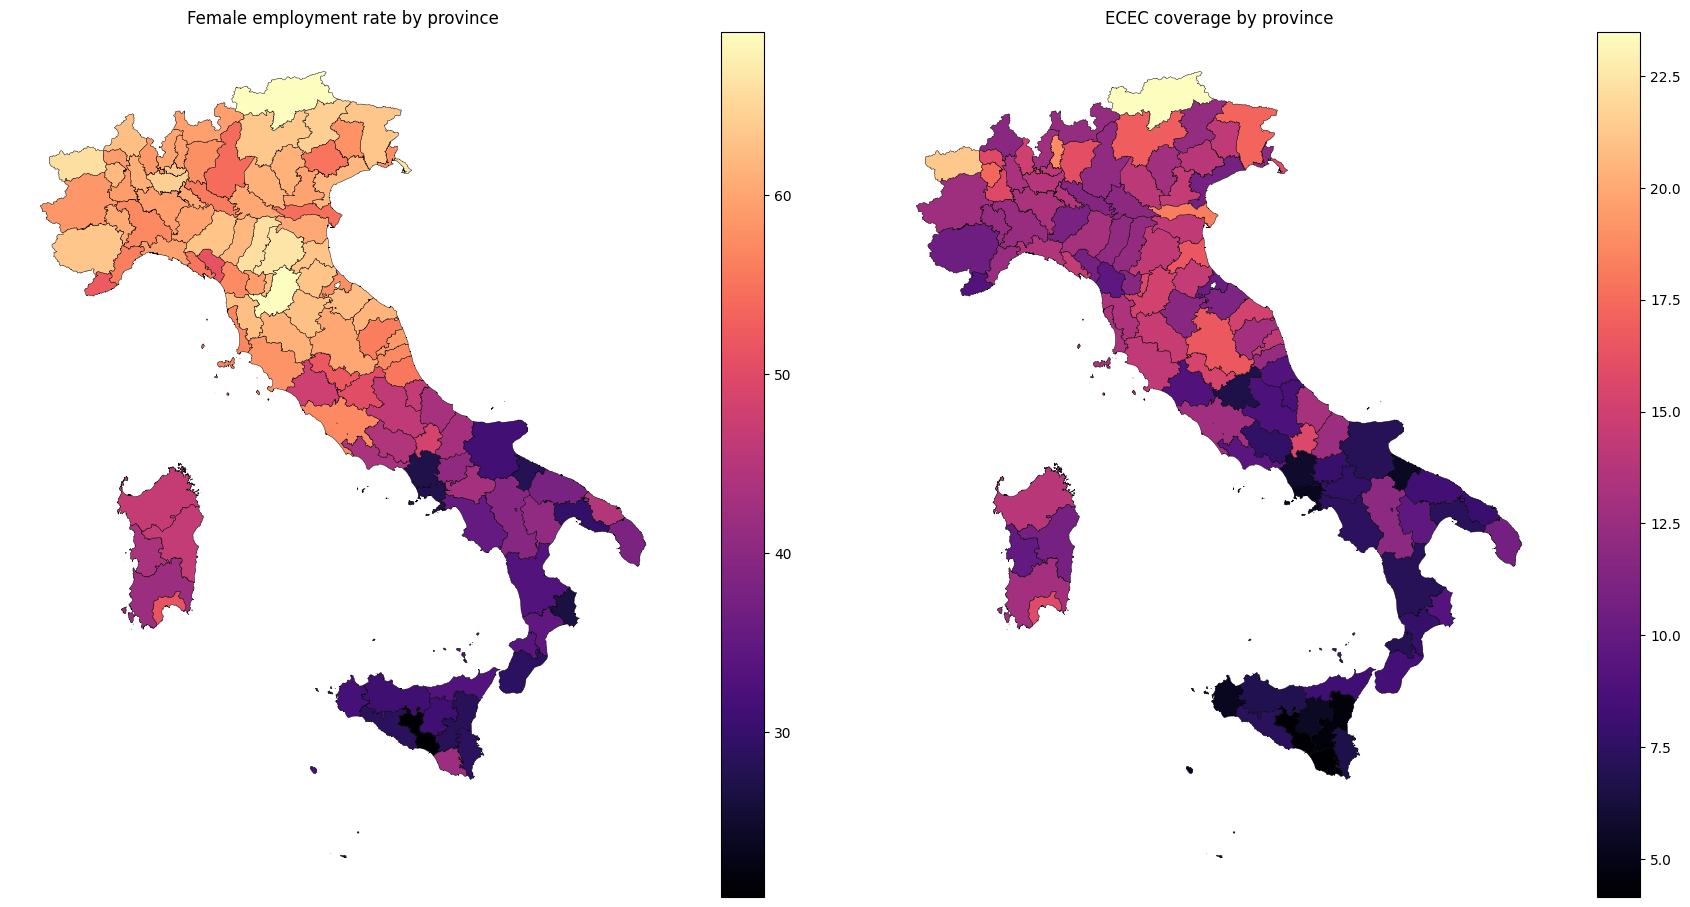
\includegraphics[width=0.9\linewidth]{chapters/images/fem_emp_rate_and_ECEC_map.png}
    \caption{Female employment rate (left) and ECEC coverage (right) by province heatmaps.}
    \label{fig:heatmap1}
\end{figure}

The heatmap clearly reveals two distinct regions, corresponding to Northern and Southern Italy. While the North exhibits peaks of women's employment reaching up to $69.1\%$, the South displays substantially lower values, with rates dropping to as low as $20.8\%$. Despite the relatively better performance of the North, Italy overall continues to record one of the lowest female employment rates in Europe.\\
The same holds for the coverage of ECEC services.\\

A positive association between women's employment and ECEC service indicators is suggested by visual inspection of the data and is formally confirmed by correlation analysis. We first compute a correlation matrix for the main employment and ECEC variables, and subsequently extend the analysis to all variables in the dataset. The results consistently indicate a strong positive correlation between women's employment rates and the provision and use of ECEC services. In particular, \texttt{fem\_empl\_rate} exhibits strong positive correlations with \texttt{per\_capita\_user\_contribution} (municipal expenditure per child financed by user contributions), \texttt{per\_capita\_public\_expenditure} (public expenditure per child), \texttt{coverage}, and \texttt{ecec\_participation} (percentage of children using ECEC services).\\

As exploratory measures of spatial autocorrelation, we compute Moran’s I (MI) \citep{Moran1950}, a global indicator ranging from $-1$ to $1$, where negative and positive values indicate negative and positive spatial autocorrelation, respectively. Statistical significance is assessed via a permutation test. For our variables of interest, we obtain $\text{MI} = 0.87$ for \texttt{fem\_empl\_rate} and $\text{MI} = 0.57$ for \texttt{coverage}, both indicating strong and statistically significant positive spatial autocorrelation.\\

To further investigate localized patterns of spatial dependence, we plot the Local Indicators of Spatial Association metric (LISA) using the local Moran's I \citep{Anselin1995} and generate cluster maps for the two variables, shown in Figure~\ref{fig:LISA}. The local Moran's I is a decomposition of the Global Moran's I statistic into individual values computed as: 

\begin{equation}   
    I_i = \frac{(Y_i - \bar Y)}{\sum_{j=1}^n (Y_i - \bar Y)^2/(n-1)}\sum^n_{j=1}w_{ij}(Y_j-\bar Y),
\end{equation}

where $Y_i$ is the value of a variable $Y$ in location \textit{i}, $\bar Y$ is the mean of $Y$, $n$ is the number of observations and $w_{ij}$ is the spatial weight between unit \textit{i} and \textit{j}. From the local Moran's I, we can check for the presence of clusters. Specifically, High--High (HH) and Low--Low (LL) clusters identify spatial concentrations of similarly high or low values (hotspots and coldspots, respectively), while High--Low (HL) and Low--High (LH) configurations indicate spatial outliers, where a province’s value contrasts with that of its surrounding area. This local analysis complements the global Moran’s I by highlighting heterogeneous spatial structures that are not captured by a single summary measure.\\

\begin{figure}[h] % THIS IMAGE LOOKS BLURED, WE NEED TO FIND A BETTER ONE
    \centering
    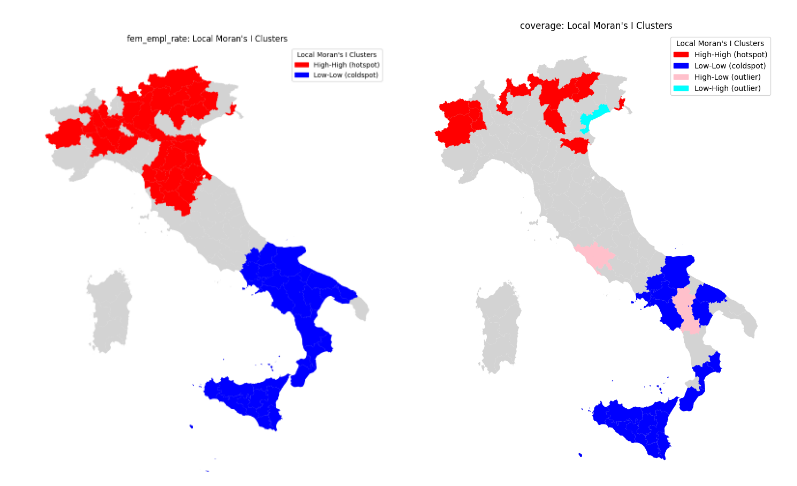
\includegraphics[width=0.9\linewidth]{Images/morans_clusters_inverted.png}
    \caption{LISA cluster map of \texttt{fem\_empl\_rate} (left) and \texttt{coverage} (right).}
    \label{fig:LISA}
\end{figure}
